\documentclass{article}

%package setup
\usepackage{graphicx}
\usepackage{amsmath}
\usepackage{fancyhdr}
\usepackage[margin=1in]{geometry}
\usepackage{comment}
\usepackage{placeins}
\usepackage{parskip}
\usepackage{subcaption}
\usepackage{appendix}
\usepackage{soul}
\usepackage{comment}
\usepackage[hidelinks]{hyperref}
\usepackage{matlab-prettifier}
\usepackage{minted}
\usepackage{enumitem}
\usepackage{float}
\usepackage{textcomp, gensymb}
\usepackage{caption}


\pagestyle{fancy}
\fancyhf{} % Clear header/footer settings
\rhead{\thepage} % Page number on the right in the header
\lhead{ASE375 Lab Report 8} % Your lab report title on the left

\begin{document}

\begin{titlepage}
  \centering
  
\includegraphics[width=10cm]{ase-logo-formal.png}  % Adjust the width as needed
  \vspace{1cm}  % Add some vertical space
 
  \Large \textbf{ASE 375 Electromechanical Systems}\\
  \large \textbf{Section 14115}\\
  \vspace{0.5cm}
  \textbf{Monday: 3:00 - 6:00 pm}\\
 
  \vspace{1cm}
 
  \hrule
  \vspace{0.5cm}
 
  \Huge \textbf{Report 8:\\
    Landing Gear Drop Test}\\
  \Huge \textbf{}\\
 
  \vspace{0.5cm}
  \hrule
 
  \vspace{1cm}
 
  \normalsize \textbf{Andrew Doty, Andres Suniaga, Dennis Hom}\\
  \normalsize \textbf{Due Date: 04/08/2024}
 
\end{titlepage}
\newpage

\tableofcontents
\thispagestyle{empty}
\newpage

\section{Introduction}
In this experiment we take a look at the transient response of a landing gear as it is dropped from various heights. Drop tests are a useful measure to verify the performance and safety of an aircraft. In this lab we use a small scale landing gear equipped with a rotary potentiometer to measure the angle of the landing gear linkage and a piezoelectric accelerometer to measure the acceleration of it's response.
\vspace{2.5mm}

Using a laser pointer and a photo-diode, we are able to perform triggered data acquisition of the transient response of the landing gear as it makes impact with the table surface. These triggered measurements allow us to gather consistent and time-resolved data for each drop height.

\section{Equipment}
Measurement devices and hardware used in this lab include:
\begin{itemize}

\item Small-Scale Landing Gear: 
\vspace{1mm}

Scaled-down 

\vspace{2.5mm}

\item Piezoelectric Accelerometer:
\vspace{1mm}

\vspace{2.5mm}

\item Laser Pointer (Red, $\gamma \approx 700\; \text{nm}$)
\vspace{1mm}

\vspace{2.5mm}


\item DAQ, NI-9215 Voltage Input Module \hyperlink{datasheets}{[1]}, NI-9263 Analog Output Module \hyperlink{datasheets}{[6]},  and LabVIEW:
\vspace{1mm}

Data Acquisition System used to process sample measurements into digital data for the computer to read.\\[5pt]
NI-9215 is an analog input module used to measure the output voltage signals of the sensors.\hyperlink{datasheets}{[3]}.\\[5pt]
LabVIEW used to model these output voltages read from the DAQ of the...

\item Solderless Breadboard, Jumper Wires, $1\; \text{k}\Omega$ Resistor, $0.1\; \micro\text{F}$ Capacitor, a Diode, and $10\; \text{k}\Omega$ Resistor: 
\vspace{1mm}

Used to make connections to the input analog modules and to construct circuits. ...

\end{itemize}

\section{Procedure}
Before beginning the experiment, setup the LabVIEW model to output the data from the photo-diode, potentiometer, and piezoelectric accelerometer:

\begin{figure}[H]
    \centering
    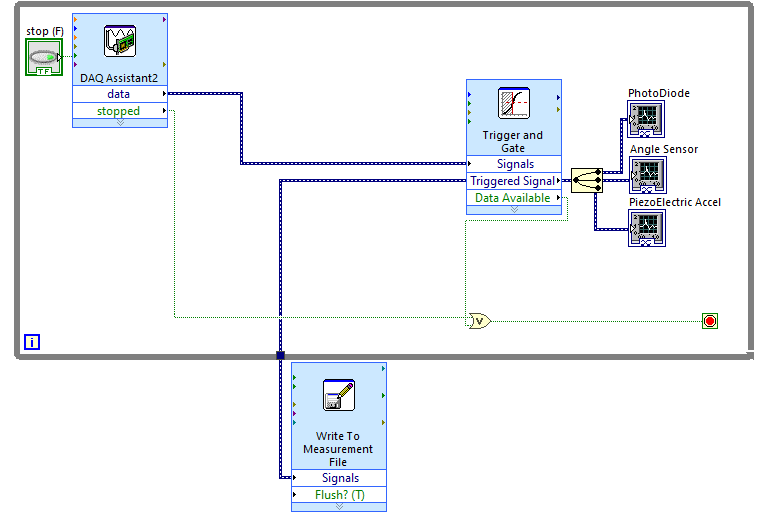
\includegraphics[width=0.65\textwidth]{lab8images/lab8blockdiag.PNG}
    \caption{LabVIEW Experiment Setup}
    \label{fig:labview}
\end{figure}

\subsection{Drop Testing}
\begin{enumerate}
    \item 
\end{enumerate}

\hypertarget{datapro}{}
\section{Data Processing}
\subsection{Variables and Equations}  

Gain of the AD623 Instrumentation Amplifier:
\begin{equation}
    G = 1 + \dfrac{100\, \text{k}\Omega}{R_{G}}
\end{equation}

Variables:
\begin{itemize}
    \item \(R_{G}\): Resistance of Gain setting resistor
\end{itemize}
\vspace{5mm}

Differential Voltage, Output Voltage (read by DAQ) is amplified by Gain $G$:
\begin{equation}
    V_{\text{OUT}} = GV_{0}
\end{equation}

Variables:
\begin{itemize}
    \item \(V_{\text{OUT}}\): Output voltage read by DAQ
    \item \(V_{0}\): Input voltage going into Instrumentation Amp
\end{itemize}
\vspace{5mm}

Harmonic Motion Equations:
\begin{equation}
    x(t) = A\sin{(\omega t)}
\end{equation}
\begin{equation}
    \ddot{x}(t) = -A\omega^{2} \sin{(\omega t)}
\end{equation}

With these harmonic motion equations we can make the estimation:
\begin{center}
    \(|x| = A\), \hspace{10mm} \(|\ddot{x}| = A\omega^{2}\), \hspace{10mm} \(\implies |x| = \dfrac{|\ddot{x}|}{\omega^{2}}\)
\end{center}

Variables:
\begin{itemize}
    \item \(x(t)\): Displacement as a function of time
    \item \(\ddot{x}(t)\): Acceleration as a function of time
    \item \(A\): Amplitude
    \item \(\omega\): Frequency
\end{itemize}
\vspace{5mm}

    
\section{Results and Analysis}

 
\section{Conclusion}



\newpage
\thispagestyle{empty}  % Clear header/footer
\begin{center}
	\vspace*{\fill}
	{\Huge Appendix}
	\vspace*{\fill}
\end{center}

% Start appendices
\newpage
\begin{appendices}
\pagestyle{fancy}
\renewcommand{\thefigure}{A\arabic{figure}}
\setcounter{figure}{0}

% \section*{t-Distribution Tables}
% \hypertarget{1}{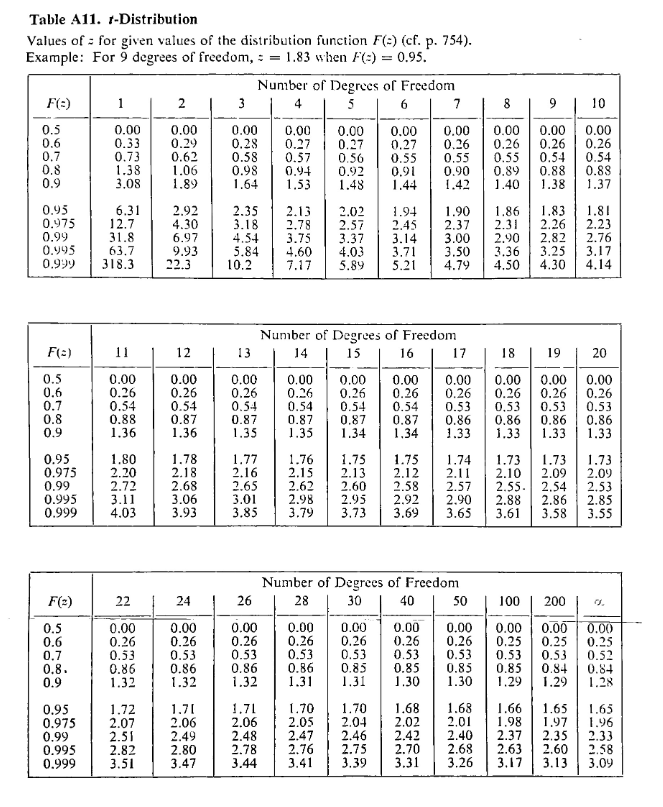
\includegraphics[width=0.95\textwidth]{t_distribution_Table_lecture3.png}}

%Add other appendix items here

\pagebreak

\hypertarget{datasheets}{}
\section{Datasheets}
\begin{enumerate}[label = {[\arabic*]}]
\item \textbf{NI-9215 Datasheet:}\\[2pt] \url{https://www.amc-systeme.de/files/pdf/ni-9215-amc.pdf}


\end{enumerate}

\end{appendices}

\end{document}
